\chapter{Fisica Medica}


\section{\textit{Lun 21 novembre - Medphys lezione 1}}
\section{Imaging medico: alcuni metodi diagnostici}

\begin{itemize}
	\item \textbf{CT (TAC in italiano)} tomografia assiale computerizzata. Si basa sui raggi X.
	\item \textbf{Risonanza Magnetica, MRI, fMRI}: possiamo generare immagini strutturali che rappresentano l'anatomia del copro umano (array tridimensionali); nel caso della fMRI possiamo acquisire questi volumi nel tempo, quindi ottenendo array 4-dimensionali.  Si basano su spin magnetici.
	\item \textbf{Nuclear (PET, SPECT)} Un tracciante radioattivo viene iniettato nel corpo umano, emette radiazione (e.g. positroni) che viene rivelata dagli strumenti.
	\item \textbf{Ultrasuoni}. Si basano su onde acustiche (ecografie).
\end{itemize}

La conoscenza dei meccanismi fisici che generano il dato su cui lavoriamo è importante.\\
Le immagini mediche non sono semplici fotografie, ma sono immagini che contengono importanti informazioni sullo stato di salute del corpo umano.\\ E' importante sempre tenere in mente che tipo di informazione può darci una determinata tecnica di imaging, per non tirar fuori informazioni che in un dataset non ci sono.

\begin{figure}[ht]
	\centering
	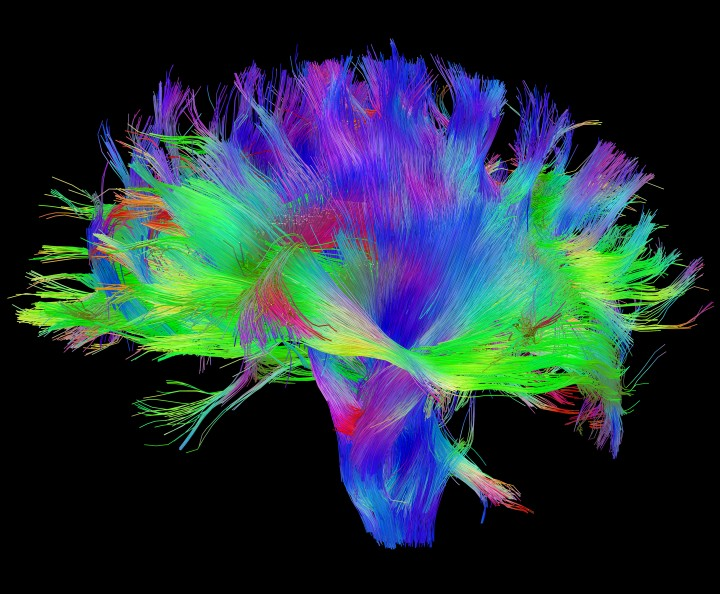
\includegraphics[width=0.45\linewidth]{figure_med/White-Matter-Fibers.jpg}
	\caption{Fibre assonali che costituiscono la materia bianca cerebrale \url{http://www.humanconnectomeproject.org/}}
\end{figure}
\FloatBarrier

Le immagini mediche riflettono diverse proprietà fisiche del corpo umano. Esse sono ottenute dall'interazione tra radiazione/ultrasuoni con i tessuti/organi.\\
Inoltre, tipicamente le immagini mediche non si limitano a 2D, ma solitamente abbiamo almeno 3 dimensioni.\\

Le immagini mediche permettono di studiare:
\begin{itemize}
	\item la struttura dei tessuti/organi
	\item la funzione dei tessuti/organi
\end{itemize}

\section{Le principali modalità di imaging diagnostico}
Quando si parla di radiografia tipicamente ci si riferisce a immagini 2D.\\
Tomografia invece si rifersice a immagini 3D.\\

\begin{figure}[ht]
	\centering
	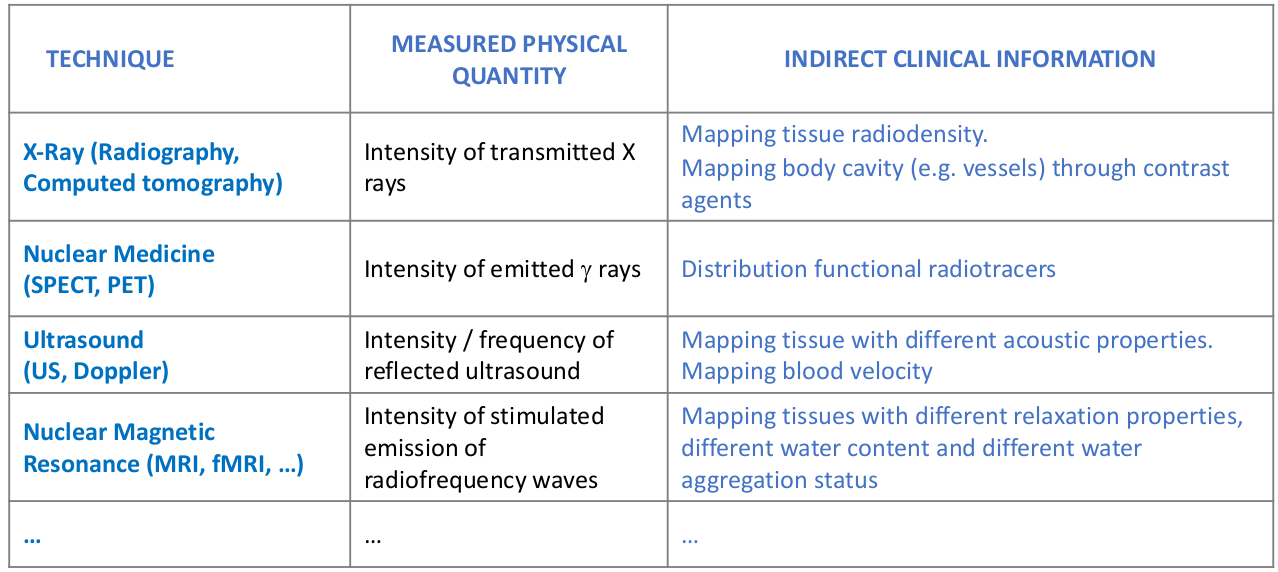
\includegraphics[width=0.9\linewidth]{figure_med/diagnostic}
\end{figure}
\FloatBarrier

Lo sforzo moderno è quello di creare dispositivi multimodali, che investigano il corpo umano da diversi punti di vista. Acquisire informazioni complementari attraverso le diverse modalità contemporaneamente. Unendo le informazioni possiamo ottenere una diagnosi più accurata.\\
Ogni tecnica ha una specifica risoluzione spaziale. TAC e Risonanza magnetica strutturale hanno una risoluzione buona (millimetrica/sub-millimetrica ), mentre le tecniche di medicina nucleare come PET e SPECT, rappresentano il metabolismo degli organi, ma con una risoluzione spaziale meno buona (ordine di qualche mm). Combinando le varie tecniche possiamo ottenere più informazioni utili.\\
 
\textbf{Medicina di precisione}: creare un trattamento specifico per ogni paziente. A contrapporsi ad un metodo basato su protocolli, come si fa attualmente nel nostro sistema sanitario.\\
Mettendo insieme tutte le informazioni sul paziente si può arrivare a delle diagnosi e a dei trattamente altamente personalizzati.\\
Sfida: come integrare i dati che vengono da sorgenti diverse in maniera efficiente.\\

\section{Il ruolo dei computer nell'imaging medico}
Da sempre i computer hanno un ruolo fondamentale nell'imaging medico.\\
I dati \textit{raw} devono essere interpretati ed elaborati attraverso algoritmi di ricostruzione per poterli poi fornire al medico. Tra le altre cose, si usano anche algoritmi di denoising basati sull'intelligenza artificiale.\\

\begin{figure}[ht]
	\centering
	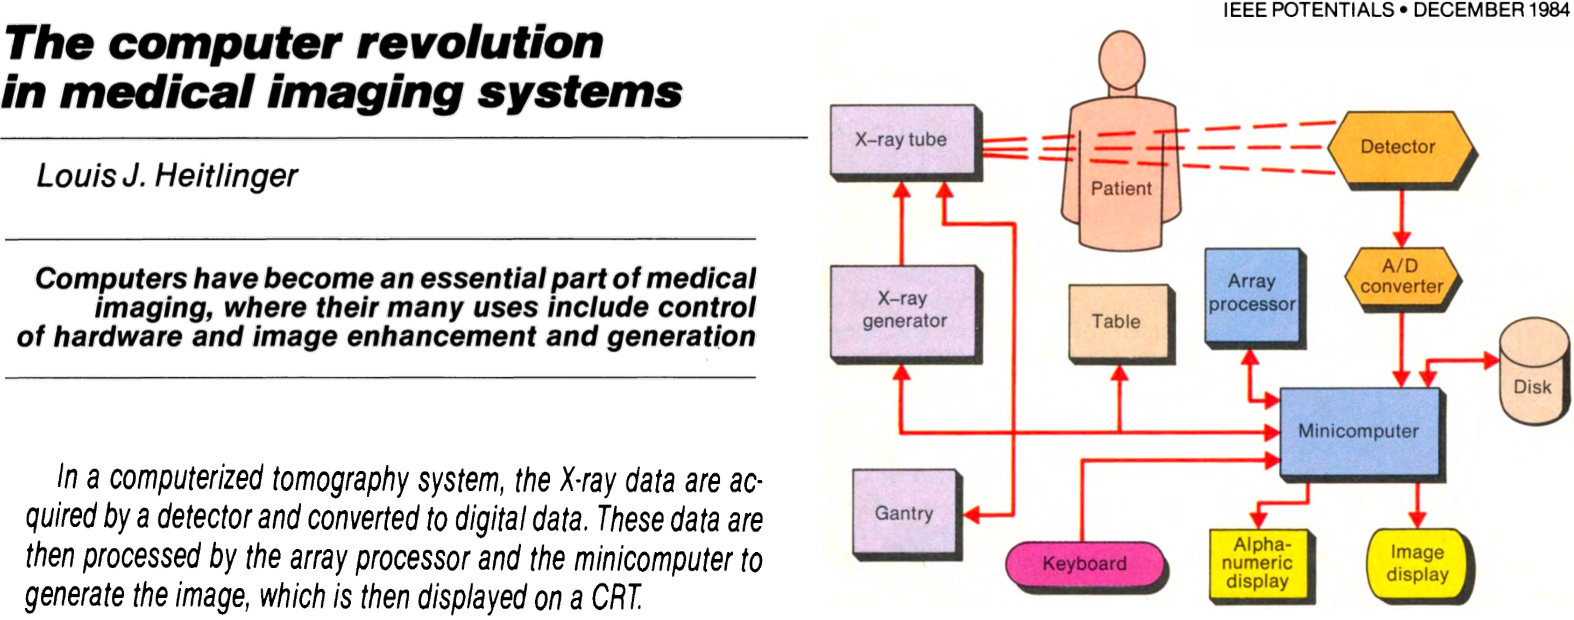
\includegraphics[width=1\linewidth]{figure_med/computers}
\end{figure}
\FloatBarrier


\begin{figure}[ht]
	\centering
	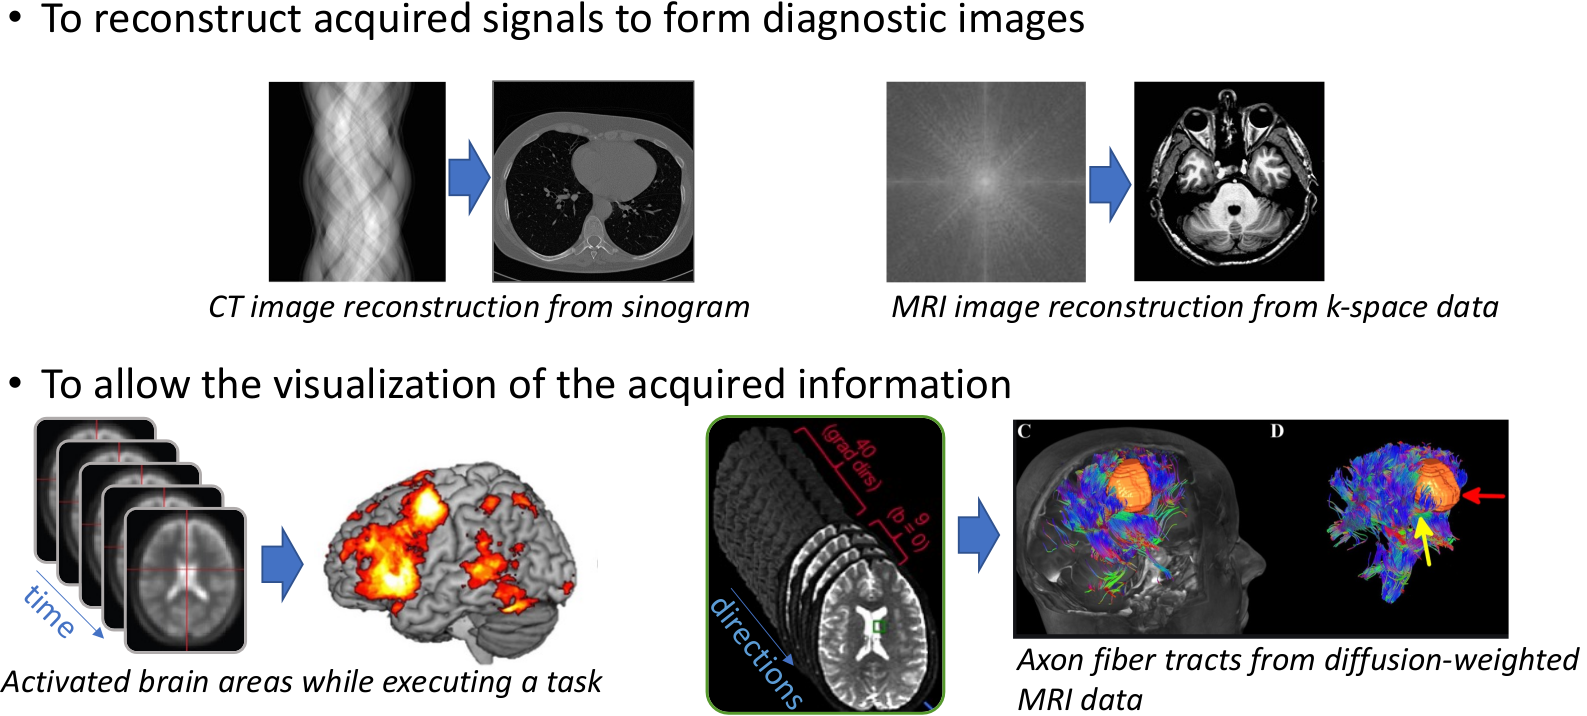
\includegraphics[width=1\linewidth]{figure_med/computer_role}
\end{figure}
\FloatBarrier

\begin{figure}[ht]
	\centering
	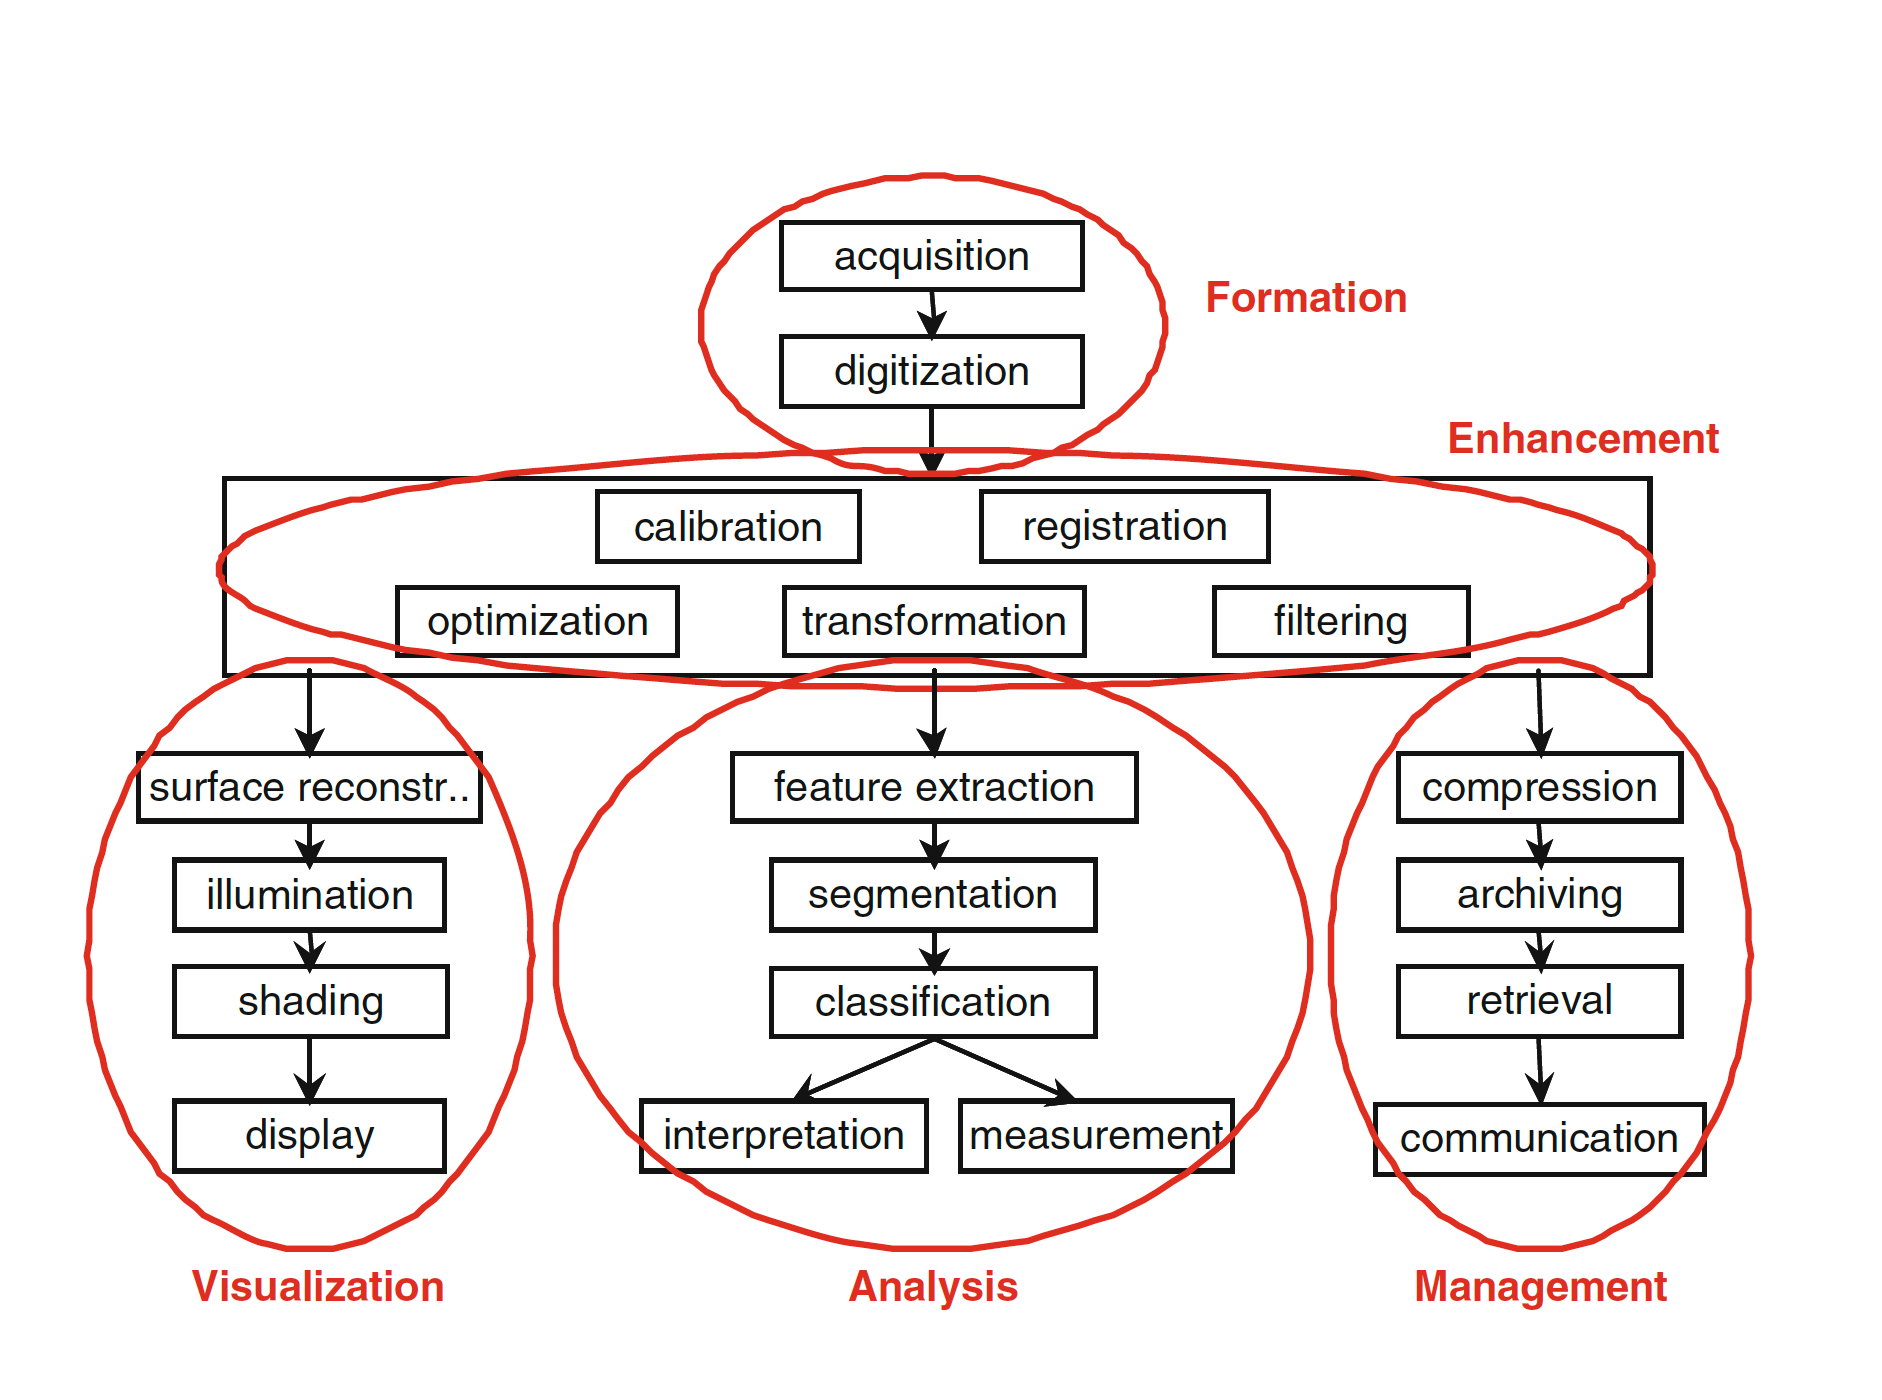
\includegraphics[width=0.85\linewidth]{figure_med/computers_med_img}
	\caption{Algorithms for
		information processing enter at many levels in the image formation	pipeline. We will focus in this
		course on the high-level Analysis procedures, and
		we will not cover the countless other possibilities}
\end{figure}
\FloatBarrier
In questo corso: a partire dall'immagine medica acquisita (già con valore diagnostico per un medico), possiamo lavorarci sopra per acquisire informazione. Ad esempio mettendo su degli algoritmi di classificazione.\\

\section{Biomedical image processing and analysis}

Il nostro obiettivo è identificare delle anomalie nelle immagini. Identificare lo stato di avanzamento di una certa lesione, per studiarne il tasso di crescita.\\
Vorremmo costruire uno strumento che sia il più robusto possibile ad una serie di variabilità a cui è esposta la lettura del medico, e che sia \textbf{riproducibile}, in modo da affiancare il medico nel processo decisionale.\\
E' importante individuare quali sono le principali fonti di incertezza!

The main objectives are:
\begin{itemize}
	\item To detect abnormalities in diagnostic images (lesions, etc.)
	\item To follow up pathological conditions (e.g. measuring the growth rate of lesions)
	\item To assess treatment efficacy
\end{itemize}

The aim is to assist clinicians in their tasks,
not to replace them: \textit{Computer Aided Detection/ Diagnosis (CAD) systems/ Decision Support Systems (DSS)}

Historical development of CAD systems:
\begin{enumerate}
	\item ’90 - Old-fashion systems (Rule-based decision systems)
	\item 2000-today - Hand-crafted feature and Machine Learning classification
	\item since 2016 - Deep Learning-based data/image classification
\end{enumerate}


\section{Data dimensionality: 3D images}

Dal sinogramma (Il sinogramma in TC è la rappresentazione bidimensionale della lettura dell'intera striscia di detettori nel tempo di rotazione attorno al paziente) lavoro con degli algoritmi di ricorstruzione, da cui poi posso ricavare delle immagini (a fette) che rappresentano l'anatomia del paziente.

(micronodulo polmonare)\\


\begin{figure}[ht]
	\centering
	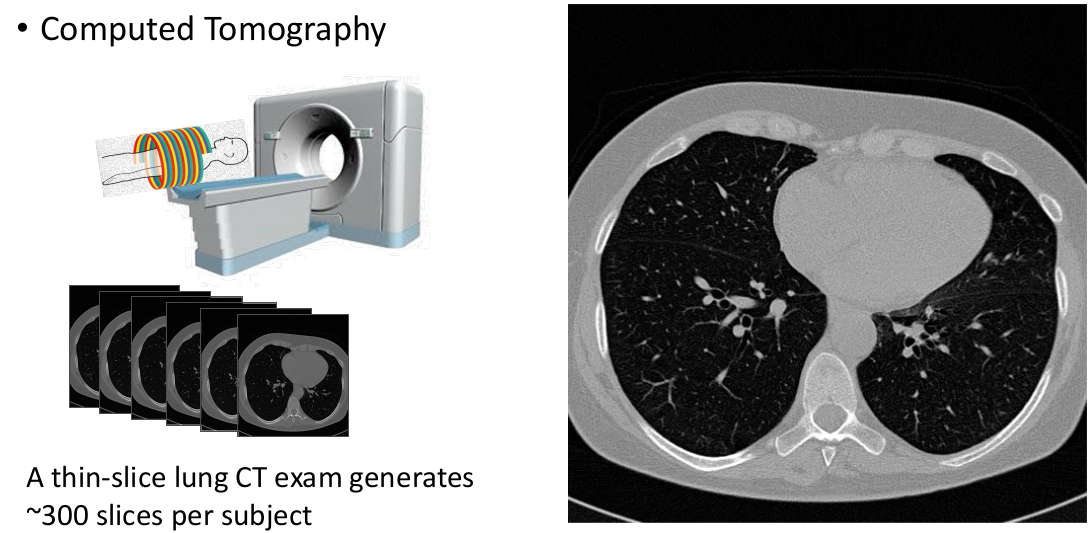
\includegraphics[width=0.7\linewidth]{figure_med/datadim3d}
	\caption{Il pixel dela TAC è di circa mezzo millimetro. I micronoduli sono dell'ordine di 5 mm.Il parenchima polmonare appare nero, i punti bianchi corrispondono a vasi sanguigni. I noduli hanno densità simile a quella dei vasi. Per capire se un punto bianco è un nodulo, bisogna vedere se compare e scompare alla presentazione di una sequenza d i varie fette.}
\end{figure}
\FloatBarrier

\section{Volume display planes}
Una TAC del torace è un volume tridimensionale.\\

%Medical images are usually displayed by anatomical planes.

\begin{figure}[ht]
	\centering
	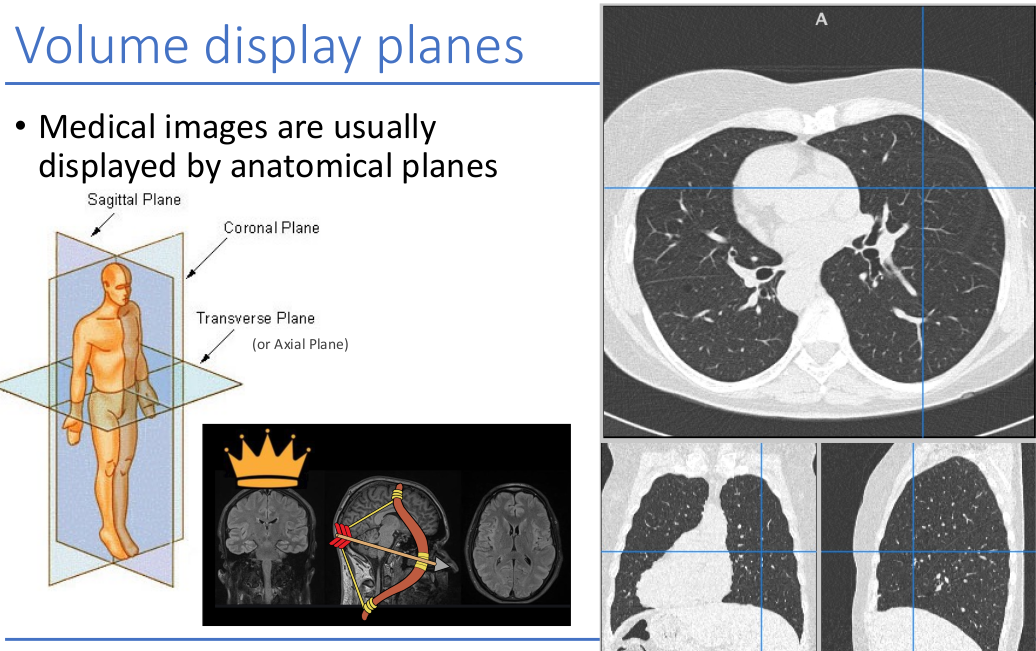
\includegraphics[width=0.8\linewidth]{figure_med/vdp}
\end{figure}
\FloatBarrier

\section{Data dimensionality: 3D and more…}

\begin{figure}[ht]
	\centering
	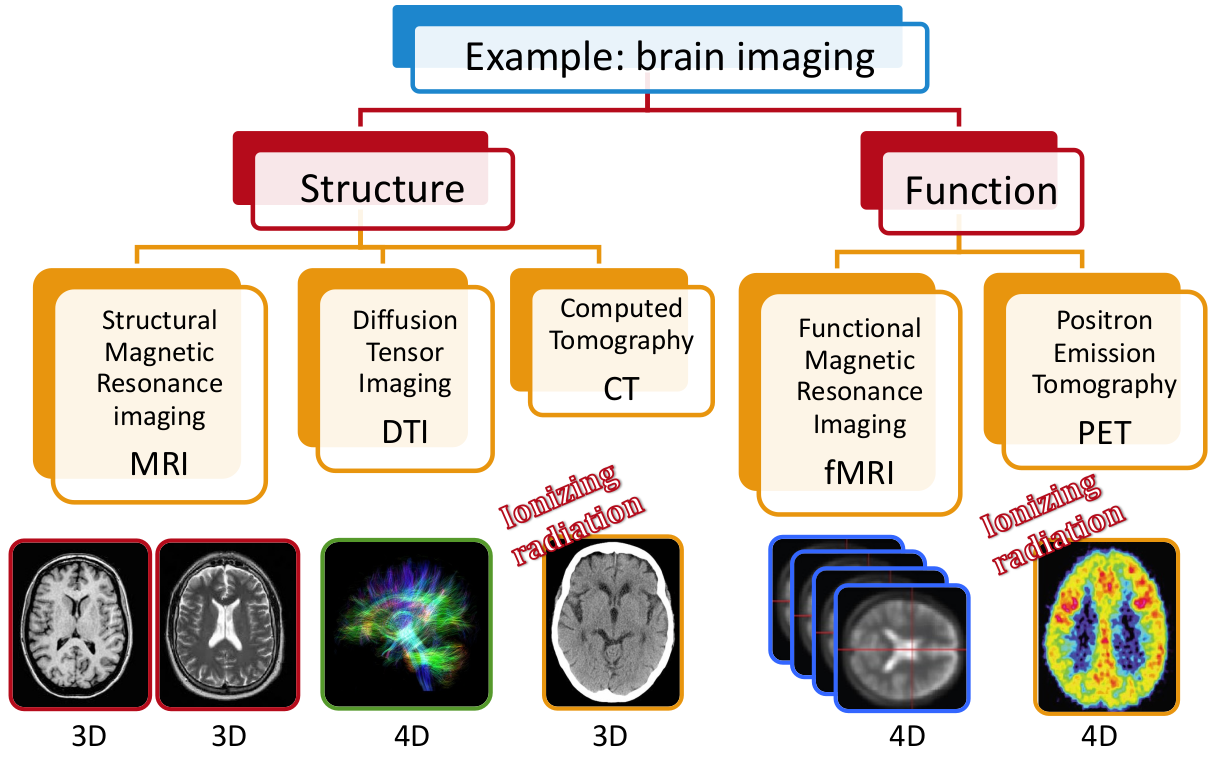
\includegraphics[width=0.9\linewidth]{figure_med/data_dim}
	\caption{La risonanza ci può dare sia informazioni strutturali, che informazioni funzionali sugli organi. Modalità diverse danno informazioni diverse, a seconda di cosa sto cercando dovrò utilizzare la tecnica appropriata. }
\end{figure}
\FloatBarrier 

\section{Structural MRI $T_1$ -weighted images}

\begin{figure}[ht]
	\centering
	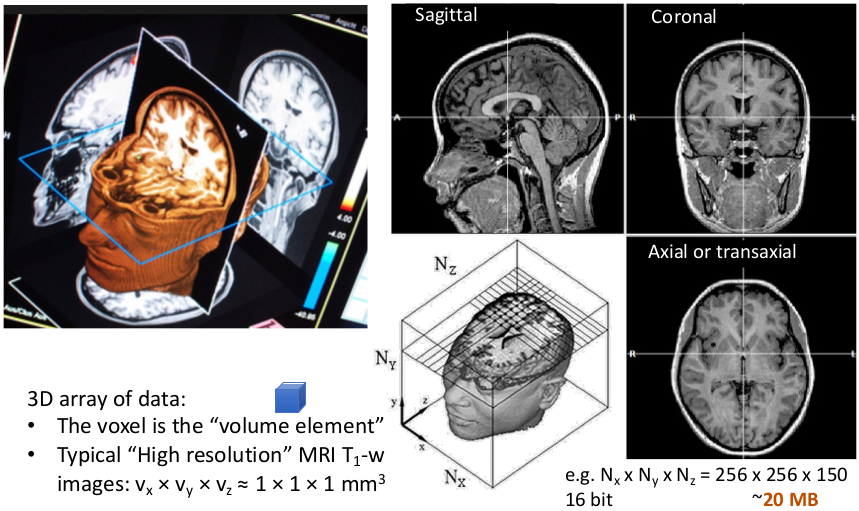
\includegraphics[width=0.8\linewidth]{figure_med/t1}
	\caption{Tipicamente si cerca di avere voxel isotropici (stesse dimensioni in x,y,z), in realta, siccome molte acquisizioni avvengono in \textit{slice} non sempre la risoluzione lungo x,y è uguale a quella lungo z.}
\end{figure}
\FloatBarrier

\newpage

\section{Functional MRI (fMRI)}


\begin{figure}[ht]
	\centering
	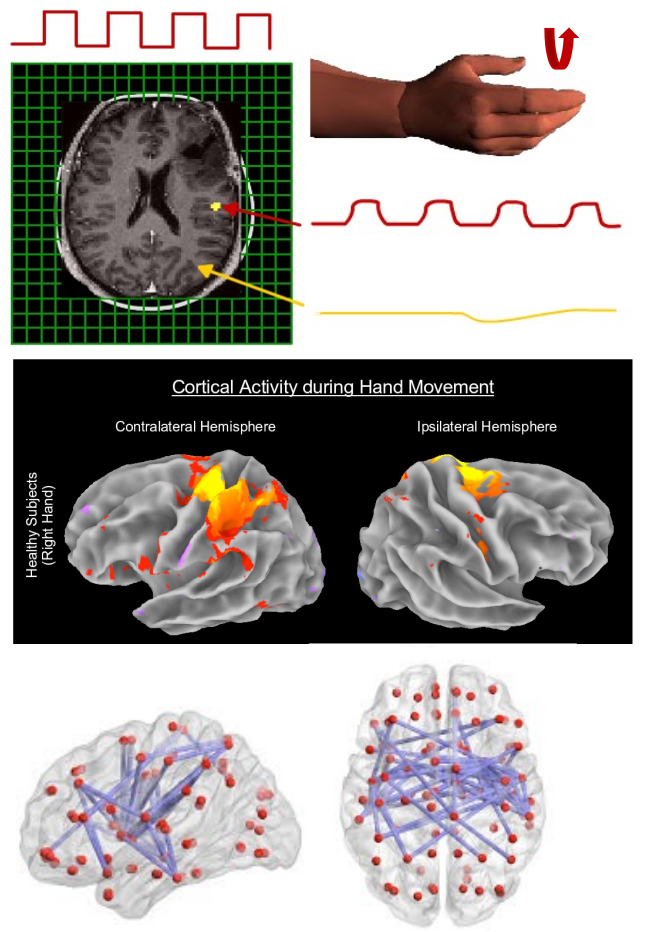
\includegraphics[width=0.65\linewidth]{figure_med/fmri}
	\caption{Posso studiare il singolo voxel al variare del tempo. POsso studiare quale regione si attiva in seguito a una certa azione.}
\end{figure}
\FloatBarrier

\begin{itemize}
	\item BOLD Response: blood-oxygen-level-dependent (BOLD) contrast. (Quando facciamo un'azione, i neuroni consumano ossigeno, e cambiano le proprietà magnetiche della regione in cui si trovano, e quindi cambia il segnale in risonanza magnetica.)
	\item Typically, 1 volume per second (3x3x3mm$^3$ ) is
	acquired for 4-5 min
	\item Stimuli (visual, auditory, tactile, …) are
	administered to the subject during the scan
	\item Analysis of data time series to look for up-and-
	down signals that match the stimulus time
	series
\end{itemize}

\textbf{Functional connectivity}

\begin{itemize}
	\item Resting state rs-fMRI: study of temporal correlations between spatially remote neurophysiological events
\end{itemize}

\newpage

\section{Data dimensionality: 2D/3D/4D/..nD images}

\begin{figure}[ht]
	\centering
	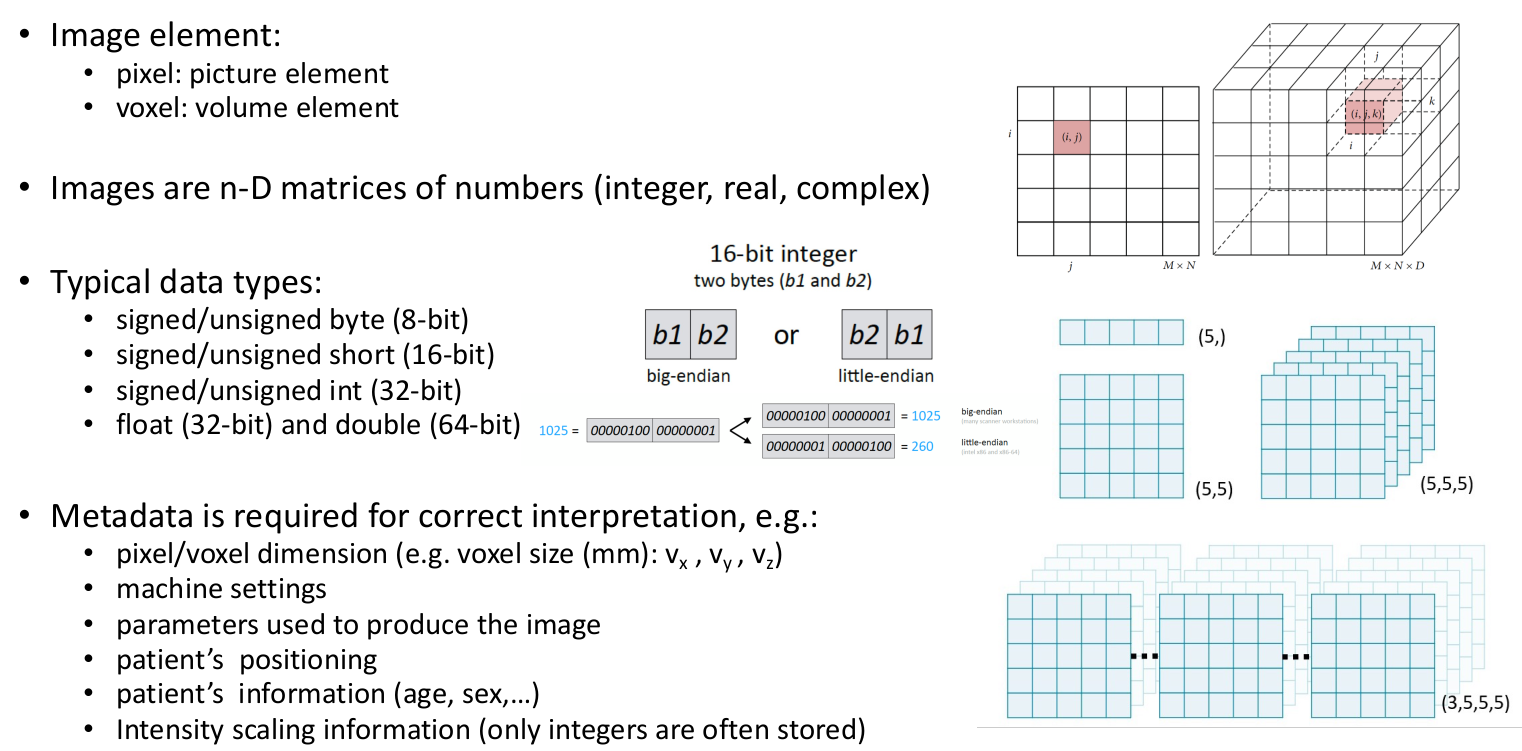
\includegraphics[width=1\linewidth]{figure_med/datadim}

\end{figure}
\FloatBarrier


L'immagine medica non è solo l'array n-dimensionale di dati. Ma deve contenere consistentemente tutte le informazioni neccassarie ad interpretare tali dati.

\section{Errors introduced by the analog to digital conversion}

\begin{figure}[ht]
	\centering
	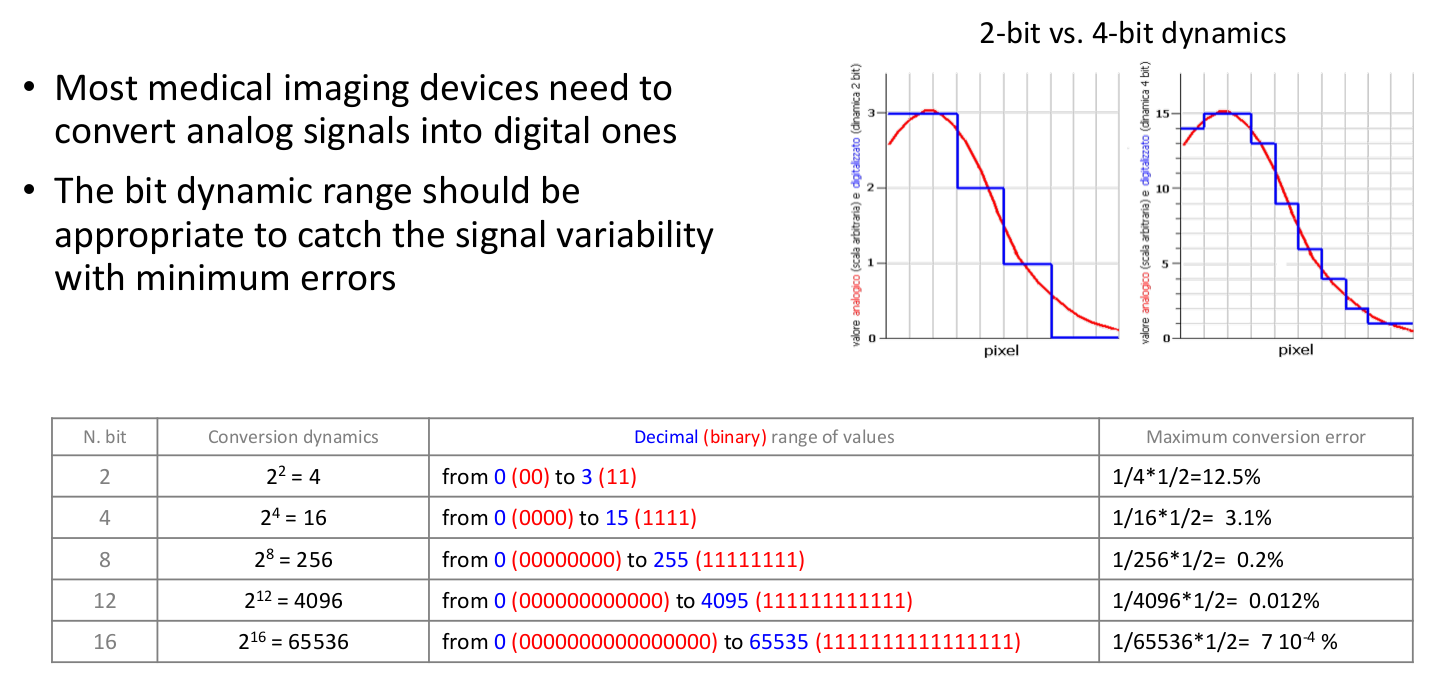
\includegraphics[width=0.8\linewidth]{figure_med/adc}
	
\end{figure}
\FloatBarrier


\section{Image representation with gray and color scales}
zz

\begin{figure}[ht]
	\centering
	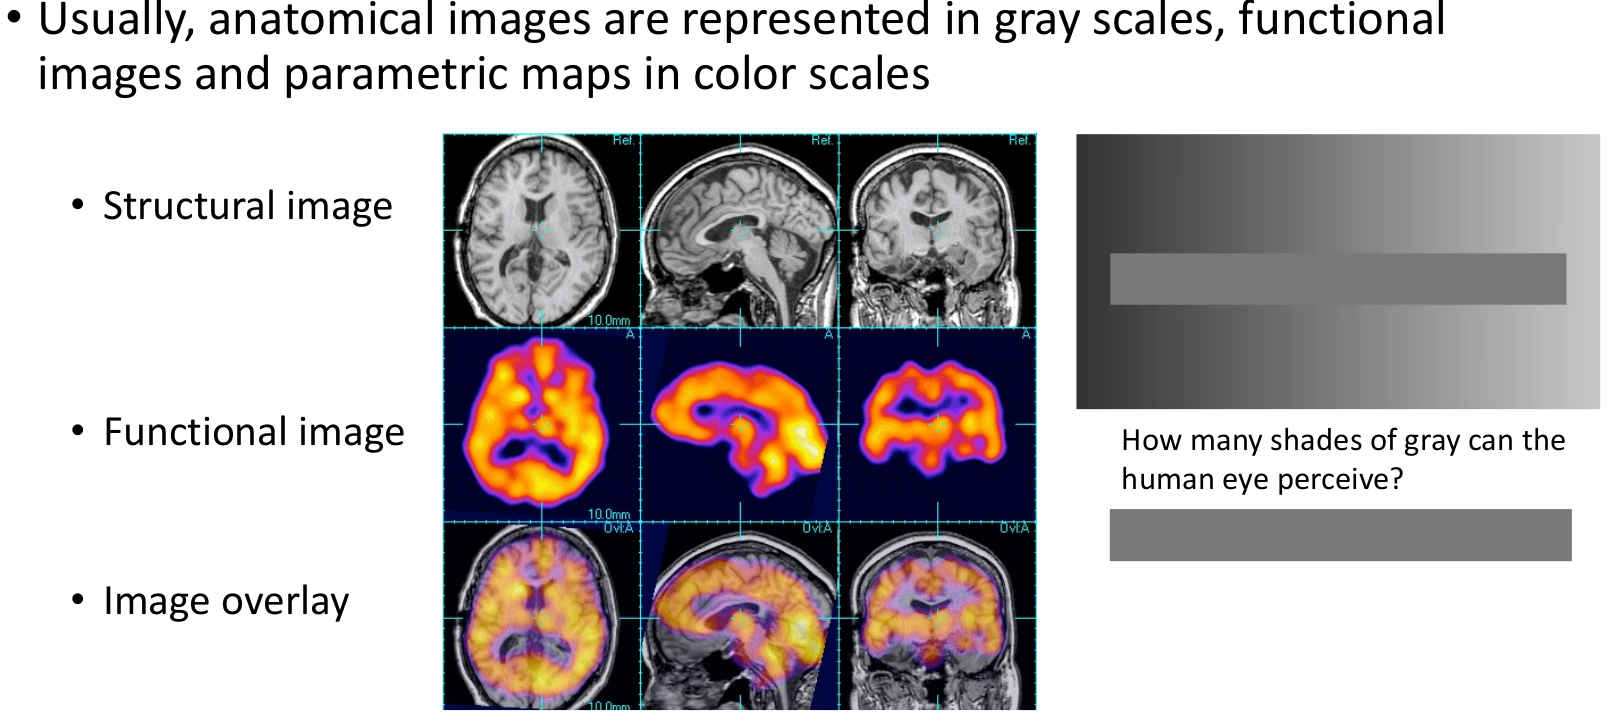
\includegraphics[width=0.8\linewidth]{figure_med/gray}
\end{figure}
\FloatBarrier

\section{Image windowing}

\begin{figure}[ht]
	\centering
	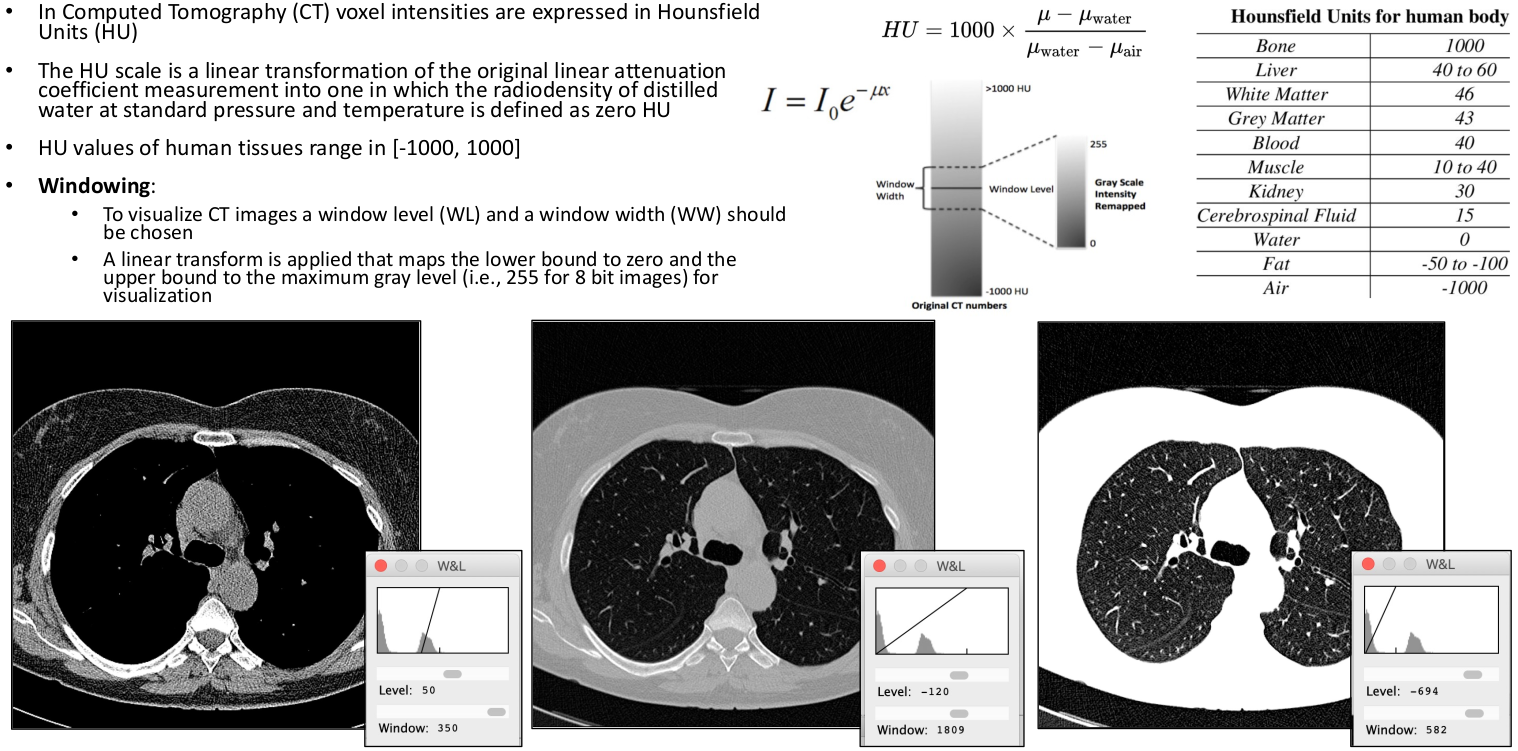
\includegraphics[width=0.9\linewidth]{figure_med/img_windowing}
\end{figure}
\FloatBarrier

\section{Look-up tables (LUTs)}

Look-up tables (LUTs) are used for pseudo coloring.
\begin{itemize}
	\item \textbf{24-bit color:} computer graphic boards typically offer 256$^3$ ($\sim$ 16 10$^6$ ) colors.
	\item \textbf{32-bit color:} supports 16 10$^6$ colors plus an alpha channel to create gradients,
	shadows, and transparencies $\rightarrow$ supports 4 10$^9$ color combinations.
	\item Pseudo coloring allows presentation of data without reducing the information as it
	would result from windowing
\end{itemize}

\begin{figure}[ht]
	\centering
	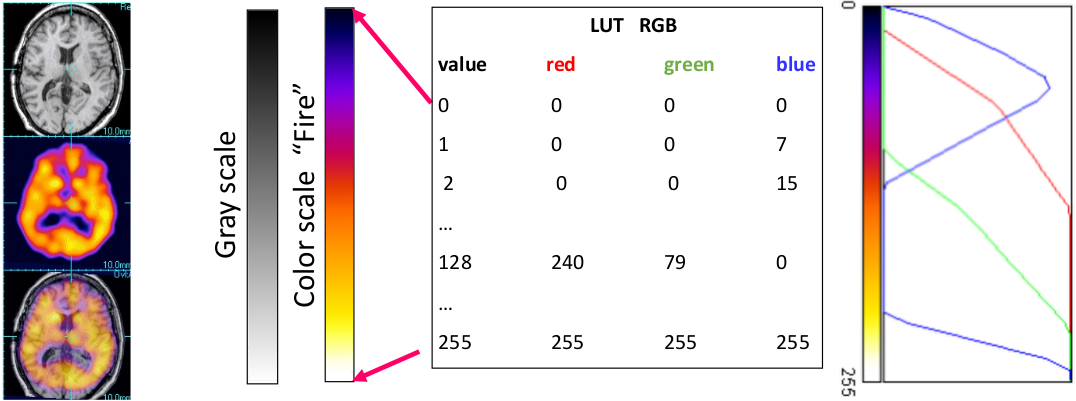
\includegraphics[width=0.9\linewidth]{figure_med/luts}
\end{figure}
\FloatBarrier

\section{Medical image file formats}

The file format describes how the image data are organized in the file and how pixel data should be interpreted by a software for correct reading and visualization.\\
Numerical values of the pixels depend on image modality, acquisition (a medical image which is separated from the context information is meaningless)

Medical image file formats belong to two categories:
\begin{itemize}
	\item Those intended to standardize images generated by different diagnostic modalities, e.g. the DICOM standard
	\item Those aiming to facilitate the post-processing analysis (e.g. NIfTI for neuroimaging)
\end{itemize}

\section{DICOM file format}
In response to the increased use of digital images in radiology the American College of Radiology (ACR) and the National Electrical Manufacturers Association (NEMA) formed a joint committee in 1983 to create a standard format for storing and transmitting medical images.\\
The committee published the original ACR-NEMA standard in 1985.\\
This standard has subsequently been revised and in 1993 it was renamed DICOM.

\begin{tcolorbox}[width=\textwidth,colback={white},title={\textbf{Di}gital Imaging and \textbf{CO}mmunication in \textbf{M}edicine (\textbf{DICOM}): },colbacktitle=cyan,coltitle=black]
	\begin{itemize}
		\item It is both a file format and communication protocol
		\item It is the standard format used in digital imaging medical devices
		\item The header and the image are contained in the same file
		\item The header contains many information on the imaging device, the acquisition parameters, the patient and the physician\\
		
		\item DICOM supports most imaging modalities
	\end{itemize}
\end{tcolorbox}

DICOM is most commonly used for storing and transmitting medical images enabling the integration of medical imaging devices such as scanners,servers, workstations, printers, network hardware, and picture archiving and communication systems (PACS) from multiple manufacturers.\\

Pixel data cannot be separated from the description of the image formation procedure: \textbf{Images should be self-descriptive}\\

The DICOM format (“anachronistically”) stores volume as a sequence of 2D slices (a 3D DICOM format exists, but it is not widespread). It is not that bad to have images stored slice by slice, as some acquisition parameters may change slice-wise during the acquisition.\\

The DICOM format only stores integer numbers as pixel values, thus a slope and an intercept to linearly transform data in the allowed range are specified.

\newpage
\subsection{DICOM metadata}

\begin{wrapfigure}{r}{0.5\textwidth}
	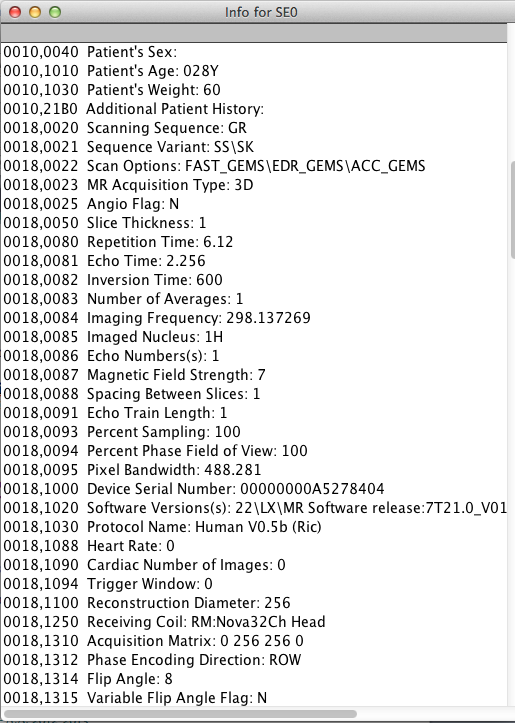
\includegraphics[width=0.5\textwidth]{figure_med/dicom_meta}
\end{wrapfigure} 


A DICOM data element, or attribute, is composed of the
following most important parts:
\begin{itemize}

\item a tag that identifies the attribute, usually in the format
(XXXX,XXXX) with hexadecimal numbers, and may be divided
further into DICOM Group Number and DICOM Element Number;
\item a DICOM Value Representation (VR) that describes the data type
and format of the attribute value (e.g. PN: Person Name; DT: Date
Time; SS: Signed Short).

\end{itemize}

Check \url{https://www.dicomlibrary.com/dicom/dicom-tags/}\\
Most fields are optional.\\
There are also vendors’ private keys.\\
Some examples:

\begin{itemize}
	\item Session Name and Study Number
	\begin{itemize}
		\item (0008, 0090) ID Referring Physician
		\item (0010,0010) Patient's Name
	\end{itemize}
	\item Image “Shape”
	\begin{itemize}
		\item (0028, 0010) IMG Rows
		\item (0028, 0011) IMG Columns
		\item (0028, 0030) IMG Pixel Spacing
		\item (0018, 0050) ACQ Slice Thickness
	\end{itemize}
	\item How and where the image data is stored
	\begin{itemize}
		\item (0028, 0100) IMG Bits Allocated
		\item (0028, 0101) IMG Bits Stored
		\item (0028, 0102) IMG High Bit
	\end{itemize}
\end{itemize}



\section{The Neuroimaging Informatics Technology Initiative (NIfTI) file format}

Another file format commonly used to store brain imaging data obtained using Magnetic Resonance Imaging methods is the Neuroimaging Informatics Technology Initiative (NIfTI).

The NIfTI stored volumes can be:
\begin{itemize}
	\item in dual file format: file.hdr, file.img
	\item in a single file: file.nii
\end{itemize}

NIfTI is the default file format of most software packages for neuroimaging post-processing: FSL, SPM, itk-SNAP, 3D Slicer, ITK \& VTK, nipy, etc.

The NIfTI format allows a double way to store the orientation of the image volume in the
space:

\begin{enumerate}
	\item rotation + translation to be used to map voxel coordinates to the scanner reference frame
	\item 12-parameter or more general transformation adopted to realign the volume to a standard template coordinate system.
\end{enumerate}

\section{Images viewers}

MANGO \url{http://ric.uthscsa.edu/mango/index.html}

\begin{figure}[ht]
	\centering
	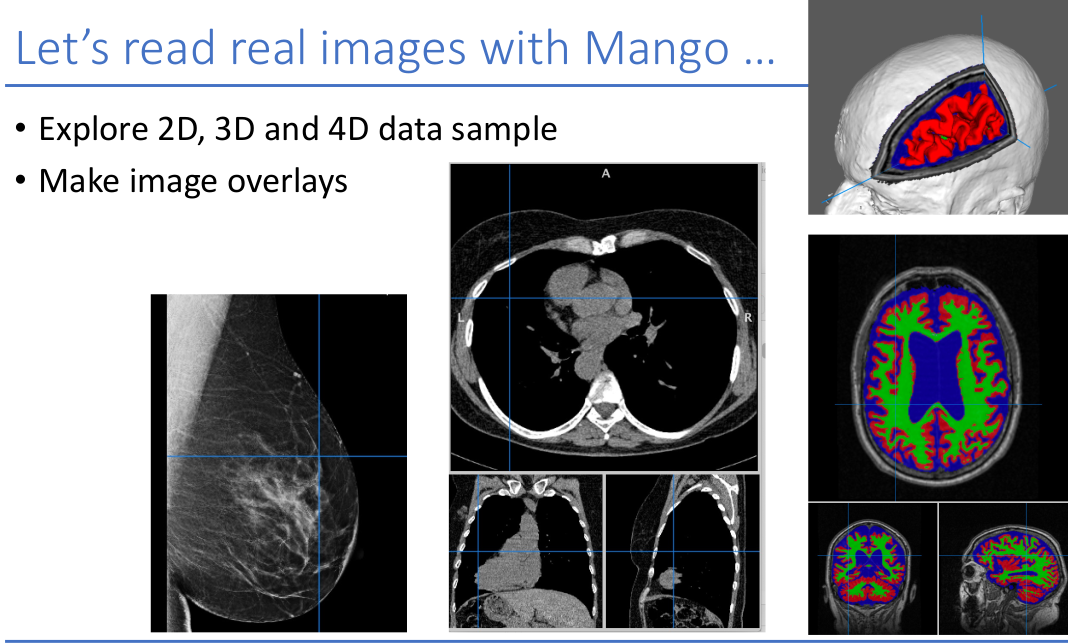
\includegraphics[width=0.9\linewidth]{figure_med/mango}
\end{figure}
\FloatBarrier

\subsection{Other medical image viewers}
- ImageJ ( \url{https://imagej.nih.gov/ij/}\\
- OsiriX (only for Mac, iPhone, iPad) \url{https://www.osirix-viewer.com}\\
- 3DSlicer \url{https://www.slicer.org}\\
- itk-SNAP  \url{http://www.itksnap.org/pmwiki/pmwiki.php}

\section{The pydicom library}

Pydicom is a pure Python package for working with DICOM files such as medical images, reports, and radiotherapy objects.\\
Pydicom makes it easy to read these complex files into natural pythonic structures for easy manipulation.\\

Requirements: numpy library is recommended, (it is only required if manipulating pixel data)\\
matplotlib is necessary to visualize data


\section{The General Data Protection Regulation (GDPR)}

The EU General Data Protection Regulation (GDPR) was approved by the EU Parliament on 14 April 2016

It is designed to:
\begin{itemize}
	\item Harmonize data privacy laws across Europe
	\item Protect and empower all EU citizens data privacy
	\item Reshape the way organizations across the region approach data privacy
\end{itemize}

GDPR and Data Science
\begin{itemize}
	\item De-identifying medical imaging is a fundamental prerequisite for data storing, processing and sharing within research projects in order to be compliant with GDPR:
	\begin{itemize}
		\item Anonymization: using the Hash function (non-reversible)
		\item Pseudo-anonymization: data is tokenized, a separate lookup file (with the original entry and
		the token) is generated and stored in a restricted database.
	\end{itemize}
\end{itemize}

\section{References and sources}
Books
\begin{itemize}
	\item The Essential Physics of Medical Imaging, Jerrold T. Bushberg
	\item Digital Image Processing for Medical Applications, Geoff Dougherty
	\item Handbook of Medical Image Processing and Analysis, Isaac N. Bankman
	\item Image Processing and Acquisition using Python, Ravishankar Chityala \& Sridevi Pudipeddi
\end{itemize}

Sources
\begin{itemize}
	\item \url{https://www.dicomstandard.org}
	\item \url{https://gdpr.eu/}
	\item\url{https://pydicom.github.io/pydicom/}
\end{itemize}

You will find the repository of course materials on \url{https://github.com/retico/cmepda_medphys}
and the image data samples to use on \url{https://pandora.infn.it/public/cmepda}
and on \url{https://drive.google.com/open?id=1YqK7ZkM-P2IrqfD7Pj-SCmjz-GWd_1-Y}

\section{Hands-On}

\url{https://github.com/retico/cmepda_medphys/tree/master/L1_code}

\newpage

\section{\textit{Mer 24 novembre - Medphys lezione 2}}

Per noi le immagini sono matrici numeriche. Per questo ci troviamo bene a lavorare con MATLAB.\\

In matlab abbiamo, oltre al formato \texttt{.m}, il formato \texttt{.mlx}, che fornisce una visualizzazione interattiva (stile jupyter notebook).

Esiste un sito dove condividere il codice con la comunità di MATLAB \url{https://it.mathworks.com/matlabcentral/fileexchange/}.\\

L'indentazione non è importante per l'interprete. E' comunque utile per rendere il codice più leggibile.

\newpage

\section{\textit{Mer lun 28 novembre - Medphys lezione 3}}